\documentclass{article}

\usepackage[dblblindworkshop]{neurips_2026}
\workshoptitle{Diffusion Language Models: Foundations, Efficiency, and Reasoning}

\usepackage[utf8]{inputenc}
\usepackage[T1]{fontenc}
\usepackage{hyperref}
\usepackage{url}
\usepackage{booktabs}
\usepackage{amsmath,amssymb,amsfonts}
\usepackage{graphicx}
\usepackage{microtype}
\usepackage{xcolor}
\usepackage{subcaption}
\usepackage{multirow}
\usepackage{nicefrac}
\usepackage{tikz}
\usetikzlibrary{arrows.meta,positioning,fit}
\hypersetup{hidelinks}

\newcommand{\pag}{PAG}
\newcommand{\rcpag}{RC-PAG}
\newcommand{\dllm}{dLM}
\newcommand{\nfe}{NFE}
\newcommand{\mask}{\mathtt{[M]}}
\newcommand{\method}{phase-adaptive generation}

\title{Phase-Adaptive Generation:\\A Stress Test of Learned Compute Scheduling for Diffusion Language Models}

\author{Anonymous Authors}

\begin{document}
\raggedbottom

\maketitle

\begin{abstract}
Diffusion language models can revise several tokens per forward call, but their practical efficiency depends on deciding how large a span to attempt and when to stop refining it. We investigate whether past refinement trajectories provide a reliable control signal. Phase-Adaptive Generation (PAG) first identifies token-level stabilization phases, then learns block-level compute from 138{,}901 AdaBlock tuples, and finally combines a categorical/ordinal history predictor with reactive delimiter boundaries. Under corrected accounting on LLaDA-8B-Instruct, PAG reduces mean model calls by 4.0\% on GSM8K and 6.7\% on MATH-500, with accuracy decreases of 1.60 and 1.33 percentage points; a block-size lookup is stronger on GSM8K. We then stress-test the idea across LLaDA and Dream using risk calibration, conservative budget ledgers, and verified macro-speculation. A cross-model policy lowers normalized calls by 9.6\% but fails its predeclared accuracy gate; output-preserving policies save below 1.3\%; and batched verification breaks exact trajectory equivalence on 22 of 64 pilot prompts. The combined evidence draws a sharp boundary: phase histories predict computational effort, but do not by themselves justify token commitment. Learned schedulers should allocate capacity while an audited, batch-invariant reference transition retains acceptance authority.
\end{abstract}

\section{Introduction}
\label{sec:introduction}

Diffusion language models generate by repeatedly revising masked positions, so one model call can advance several tokens at once. This parallelism creates a control problem absent from left-to-right decoding: how large a span should the model attempt, and how long should it refine that span before moving on? Existing decoders answer with fixed schedules or current-step confidence signals~\citep{wu2025fastdllm,lu2026adablock,mohamed2025sched}. Both are useful, but neither asks whether the trajectory itself forecasts where later compute will be needed.

Phase-adaptive generation (\pag{}) starts from a simple observation: reasoning traces are not uniformly difficult. Template text and delimiters often stabilize early, while arithmetic, variable binding, and answer finalization remain uncertain for longer. The difficult part is turning this structure into a decoder. Offline accuracy is not enough. The scheduler changes the trajectory that produces its own future features; block sizes are strongly multimodal; and a premature commitment can alter every later block. A useful predictor can therefore be a poor controller.

We study this gap from trace analysis through deployment. We first instrument Dream and LLaDA~\citep{ye2025dream,nie2025llada}, measure token stabilization, and use change-point detection (CPD) to expose local shifts in uncertainty. Because those boundaries depend strongly on the detector, we then move to 138{,}901 block-native tuples collected from AdaBlock on 5{,}000 GSM8K training problems. A categorical/ordinal Transformer predicts the next block control from recent history, while the deployed scheduler preserves AdaBlock's delimiter boundary and uses the prediction only to set a refinement budget. Finally, we stress-test increasingly conservative risk controls on LLaDA-8B-Instruct and Dream-7B instead of selecting a favorable run after the fact.

Across the experiments, corrected forward-pass accounting shows that \pag{} reduces the mean number of forward evaluations (\nfe{}) on LLaDA by 4.0\% on GSM8K and 6.7\% on MATH-500, with accuracy decreases of 1.60 and 1.33 percentage points. A size-conditioned lookup table is at least as competitive on GSM8K. A later cross-model policy lowers normalized \nfe{} by 9.6\% overall, but fails the predeclared accuracy-noninferiority gate because Dream loses substantially more accuracy. Conservative risk ledgers preserve outputs but save less than 1.3\%; batched macro-verification appears promising in physical \nfe{} yet fails exact trajectory audits. The same limitation recurs across these protocols: phase histories can forecast computational effort, but they should not decide token acceptance without verification.

\paragraph{Contributions.}
We make three empirical contributions. First, we connect token-level phase diagnostics to a block-native prediction problem and document why continuous boundary regression fails on a multimodal control space. Second, we give an audited evaluation of learned block-history scheduling, including a stronger history-free control and corrected \nfe{} accounting. Third, we report a seven-protocol, two-model stress test that separates predictive quality, task accuracy, sequential model calls, batch work, and exact trajectory equivalence. The outcome is a concrete rule for adaptive \dllm{} decoding: learn capacity allocation, retain reactive semantic boundaries, and keep commitment under an auditable token-level authority.

\section{Related work}
\label{sec:related}

\paragraph{Masked and block diffusion language models.}
Discrete and masked diffusion models replace left-to-right factorization with iterative denoising~\citep{lou2024sedd,sahoo2024mdlm}. LLaDA and Dream scale this formulation to instruction following and reasoning~\citep{nie2025llada,ye2025dream}. Block diffusion introduces a semi-autoregressive interface: the decoder completes one contiguous block before exposing it as context to the next~\citep{arriola2025block}. That interface makes block size and within-block refinement explicit controls. Our work studies whether realized block histories help set those controls; it does not change the model or training objective.

\paragraph{Adaptive and early-exit decoding.}
Fast-dLLM combines confidence transfer with KV caching and parallel decoding~\citep{wu2025fastdllm}. AdaBlock chooses semantic boundaries from delimiter confidence and adapts refinement to the active block~\citep{lu2026adablock}; it is our native decoder and strongest same-stack baseline. Adaptive Parallel Decoding (APD) learns token-wise denoising paths, whereas SchED and more recent stability rules stop from inter-step similarity or persistent predictions~\citep{israel2025apd,mohamed2025sched,mohamed2026less}. These methods establish that current-state confidence and stability are useful. \pag{} asks a different question: whether previous blocks add predictive value after controlling for a strong current-state or size-conditioned rule.

\paragraph{Risk control and verified acceleration.}
Learn-then-Test and conformal risk control provide finite-sample tools for selecting a policy under a bounded loss~\citep{angelopoulos2021ltt,angelopoulos2022crc}. We apply this machinery to a same-state premature-commitment loss, while evaluating task correctness separately. Self-speculative \dllm{} decoders instead batch draft states and verify them against a reference transition~\citep{gao2025ssd,han2026s2d2}. Our later protocols combine these ideas but also audit a systems assumption that is easy to omit: a nominally deterministic transition must remain invariant when evaluated alone or as one row of a batch. What remains unclear in this literature is whether a predictive phase signal survives both closed-loop deployment and the batch implementation of verification. Our contribution is the resulting end-to-end evidence boundary, not a claim of superiority over these contemporaneous decoders.

\section{Phase-adaptive generation}
\label{sec:method}

\pag{} has three stages (Figure~\ref{fig:pipeline}). Offline trace analysis tests whether the trajectory contains localized compute signals. Block-native traces then supervise a next-control predictor. Online, the predictor shares control with the native decoder: AdaBlock selects the semantic boundary from current logits, while \pag{} forecasts only the refinement budget. This division was fixed before the audited evaluation.

\begin{figure}[t]
  \centering
  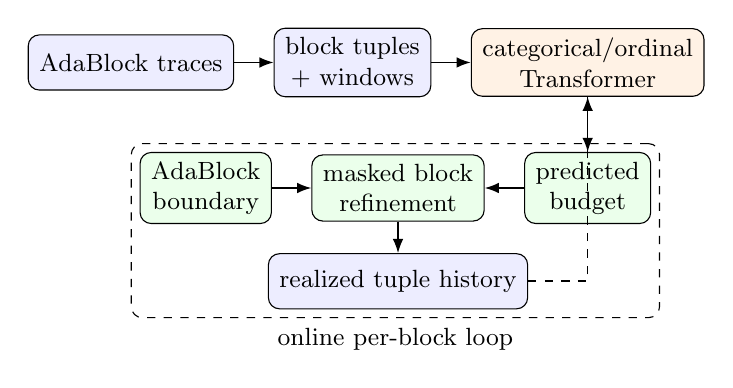
\begin{tikzpicture}[
      node distance=4mm and 5mm,
      box/.style={draw, rounded corners, align=center, minimum height=7mm,
                  inner xsep=4pt, font=\small},
      data/.style={box, fill=blue!7},
      model/.style={box, fill=orange!10},
      online/.style={box, fill=green!8},
      arr/.style={-{Latex[length=1.8mm]}, line width=.55pt}]
    \node[data] (traces) {AdaBlock traces};
    \node[data, right=of traces] (tuples) {block tuples\\+ windows};
    \node[model, right=of tuples] (predictor) {categorical/ordinal\\Transformer};
    \node[online, below=7mm of predictor] (budget) {predicted\\budget};
    \node[online, left=of budget] (refine) {masked block\\refinement};
    \node[online, left=of refine] (boundary) {AdaBlock\\boundary};
    \node[data, below=of refine] (history) {realized tuple history};
    \draw[arr] (traces) -- (tuples);
    \draw[arr] (tuples) -- (predictor);
    \draw[arr] (predictor) -- (budget);
    \draw[arr] (boundary) -- (refine);
    \draw[arr] (budget) -- (refine);
    \draw[arr] (refine) -- (history);
    \draw[arr, dashed] (history.east) -| (predictor.south);
    \node[draw, dashed, rounded corners, fit=(boundary)(refine)(budget)(history),
          inner sep=3pt, label={[font=\small]below:online per-block loop}] {};
  \end{tikzpicture}
  \caption{\pag{} separates two control signals. Current logits determine the next semantic boundary; history predicts a refinement budget. The realized tuple closes the loop only after the block is decoded.}
  \label{fig:pipeline}
\end{figure}

\subsection{Phase signals are diagnostic, not labels}
\label{sec:phase-signals}

For each output position, we record its predicted identity, top-one and top-two probabilities, and entropy after every refinement call. The stabilization time of token $i$ is the earliest step after which its identity never changes,
\begin{equation}
  s_i=\min\{t : \hat{x}_i^{(u)}=\hat{x}_i^{(T)}\ \text{for all }u\ge t\}.
  \label{eq:stabilization}
\end{equation}
We read confidence, margin, entropy, and step index at the stabilization time in Equation~\ref{eq:stabilization}, then segment each feature along token position with Pruned Exact Linear Time (PELT)~\citep{killick2012optimal}. Figure~\ref{fig:phase-data} shows the recurring pattern: long high-confidence spans are interrupted by lower-confidence computation, and block sizes concentrate on delimiter-only and default-cap modes.

The segmentation is intentionally not used as supervision. Boundaries move when the feature, smoothing window, cost, or penalty changes; representative traces yield between two and eight segments under reasonable settings. CPD therefore establishes that trajectories are structured, but does not define a stable scheduler target. The training path instead uses decisions directly observed from a block decoder.

\begin{figure}[t]
  \centering
  \begin{minipage}[c]{0.38\linewidth}
    \centering
    \scriptsize
    \setlength{\tabcolsep}{2.5pt}
    \begin{tabular}{p{0.17\linewidth}p{0.45\linewidth}r}
      \toprule
      Span & Text excerpt & Mean $p$ \\
      \midrule
      $[0,2)$ & \texttt{To solve} & .791 \\
      $[2,22)$ & \texttt{the equation\ldots} & .992 \\
      $[24,27)$ & \texttt{will follow} & .669 \\
      $[38,40)$ & \texttt{parentheses} & .401 \\
      \bottomrule
    \end{tabular}
    \vspace{2pt}

    \small (a) One PELT segmentation.
  \end{minipage}\hfill
  \begin{minipage}[c]{0.59\linewidth}
    \centering
    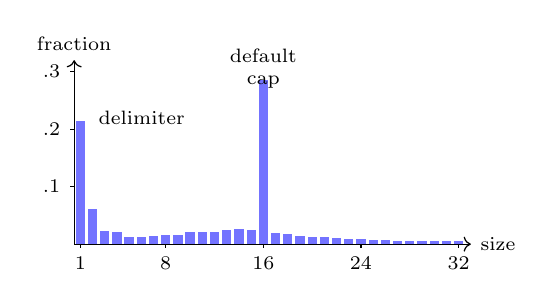
\begin{tikzpicture}[x=0.155cm,y=7.3cm]
      \draw[->,line width=.45pt] (0.5,0) -- (33,0) node[right,font=\scriptsize] {size};
      \draw[->,line width=.45pt] (0.5,0) -- (0.5,.32) node[above,font=\scriptsize] {fraction};
      \foreach \x/\y in {1/.2148,2/.0609,3/.0227,4/.0212,5/.0119,6/.0122,
        7/.0135,8/.0151,9/.0160,10/.0206,11/.0207,12/.0216,13/.0242,
        14/.0267,15/.0246,16/.2853,17/.0192,18/.0171,19/.0147,20/.0130,
        21/.0126,22/.0101,23/.0093,24/.0082,25/.0071,26/.0065,27/.0059,
        28/.0061,29/.0054,30/.0053,31/.0051,32/.0046}
        \fill[blue!55] (\x-.38,0) rectangle (\x+.38,\y);
      \foreach \x in {1,8,16,24,32}
        \draw (\x,0) -- (\x,-.006) node[below,font=\scriptsize] {\x};
      \foreach \y in {.1,.2,.3}
        \draw (0.5,\y) -- (0.15,\y) node[left,font=\scriptsize] {\y};
      \node[font=\scriptsize,align=center] at (16,.305) {default\\cap};
      \node[font=\scriptsize,anchor=west] at (1.7,.22) {delimiter};
    \end{tikzpicture}

    \small (b) Training block-size distribution.
  \end{minipage}
  \caption{From token-level phases to block-native data. (a) One algebra trace contains adjacent spans with markedly different stabilization confidence; the exact boundaries vary with detector settings. (b) The 138{,}901 training blocks form a discrete, multimodal distribution. Size 1 is dominated by delimiter blocks, while size 16 is the default content cap.}
  \label{fig:phase-data}
\end{figure}

\subsection{Block-native next-control prediction}
\label{sec:predictor}

We run AdaBlock with LLaDA-8B-Instruct on 5{,}000 GSM8K training problems~\citep{cobbe2021gsm8k}. After each decoded block, we store its size and realized \nfe{}, stabilization/refinement statistics, mean and minimum confidence, digit fraction, delimiter fraction, and gap statistics. The corpus contains 138{,}901 training tuples and 5{,}543 validation tuples. Sliding windows of eight realized tuples predict the next pair $y_t=(b_t,r_t)$, where $b_t$ is block size and $r_t$ is the refinement budget.

The target distribution rules out ordinary regression. A squared-error predictor averages the size-1 delimiter mode and the content-block mode, producing boundaries that seldom occur in the trace corpus. We instead use a Transformer encoder~\citep{vaswani2017attention} with a 128-way categorical head for $b_t$ and an 83-threshold ordinal head for $r_t$. The budget head is conditioned on the block-size logits. With categorical logits $z^b$ and ordinal logits $z^r$, training minimizes
\begin{equation}
 \mathcal{L}=\operatorname{CE}(z^b,b_t)
 +\frac{1}{83}\sum_{k=1}^{83}\operatorname{BCEWithLogits}
       \bigl(z^r_k,\mathbf{1}[r_t>k]\bigr).
 \label{eq:loss}
\end{equation}
We optimize Equation~\ref{eq:loss} with a model of hidden size 64, four heads, four layers, 0.1 dropout, and learning rate $5\times10^{-4}$; all inputs are z-score normalized with training statistics. Appendix~\ref{app:predictors} reports regression, random-forest, and architecture ablations.

\subsection{Hybrid online scheduling}
\label{sec:scheduler}

At block $t$, AdaBlock scans current logits for a high-confidence delimiter and returns the boundary $b_t$. The first block follows AdaBlock; later blocks pass the last eight realized tuples to the predictor and use only its budget $r_t$. Within the active block, masked positions are refined until the budget is reached. The decoder may then exit when all remaining predictions exceed confidence 0.8 or have stayed unchanged for two calls; a hard ceiling prevents unbounded refinement. Each initial proposal call and each refinement call counts toward \nfe{}.

This hybrid follows directly from an observed feedback failure. Letting the predictor choose both controls often selects $(b_t,r_t)=(1,1)$. The resulting trivial tuple makes another small prediction more likely, pushing the online feature distribution farther from the training corpus at every block. Preserving the reactive delimiter boundary breaks that loop. It also leaves a clean experimental question: does history forecast budget better than AdaBlock or a lookup table conditioned only on $b_t$?

\section{Evidence protocol}
\label{sec:protocol}

\paragraph{Initial audited evaluation.}
The primary \pag{} comparison uses deterministic LLaDA-8B-Instruct decoding on all 1{,}319 GSM8K test problems and a 300-example index-stratified MATH-500 sample~\citep{hendrycks2021math}. GSM8K also includes a frozen development slice for choosing among eight scheduler variants and a disjoint 919-example confirmatory complement. The comparators are AdaBlock and a history-free lookup policy that returns the median training \nfe{} for the current block size. Every method counts the boundary proposal call and all subsequent refinement calls. This corrects the legacy course result, whose \pag{} counter omitted the initial proposal and is excluded from every claim here.

\paragraph{Cross-model stress test.}
Risk-calibrated \pag{} (\rcpag{}) uses pinned LLaDA-8B-Instruct and Dream-v0-Instruct-7B revisions, temperature zero, generation length 256, at most 64 refinement calls, and block length at most 64. Estimator fitting, policy screening, and calibration use disjoint mixtures of GSM8K, MATH, and Mostly Basic Python Problems (MBPP) training data~\citep{austin2021mbpp}. Confirmation uses 500 GSM8K test, 300 MATH-500, 100 sanitized MBPP, and 100 HumanEval prompts~\citep{chen2021humaneval}; HumanEval is out of domain. Each candidate stop is compared with a same-state full-refinement shadow. A finite policy family is selected with exact binomial Learn-then-Test control at familywise level 0.05, but the certificate concerns this premature-commitment loss, not answer correctness.

\paragraph{Promotion gates and statistics.}
Results are paired by prompt. We report mean \nfe{}, exact task accuracy, and latency, with 10{,}000-sample paired bootstrap intervals where available. A cross-model policy is promoted only if it reduces \nfe{} on both models, beats the eligible history-free control, and has an accuracy-difference lower bound of at least $-2$ percentage points. Later protocols add model-wise minimum savings or exact sequence-equivalence gates. Partial screens and failed audits are reported as diagnostics, never as confirmatory wins.

\section{Results}
\label{sec:results}

\subsection{Initial PAG exposes a real trade-off}

Table~\ref{tab:initial-results} gives the corrected LLaDA result. \pag{} saves 4.0\% \nfe{} on GSM8K and 6.7\% on MATH-500, but loses 1.60 and 1.33 accuracy points. On the untouched GSM8K complement, the paired accuracy difference is $-1.20$ points with a 95\% interval of $[-2.61,0.22]$. The interval includes parity, but the point estimates do not support a dominance claim.

\begin{table}[t]
  \caption{Corrected LLaDA evaluation. Accuracy is exact-answer percentage (higher is better); \nfe{} counts all model forward calls (lower is better). The lookup baseline conditions only on block size.}
  \label{tab:initial-results}
  \centering
  \small
  \begin{tabular}{llrrr}
    \toprule
    Dataset & Method & Accuracy $\uparrow$ & Mean \nfe{} $\downarrow$ & $\Delta$\nfe{} \\
    \midrule
    \multirow{3}{*}{GSM8K ($n=1{,}319$)}
      & AdaBlock & 77.79 & 87.81 & --- \\
      & size lookup & 76.42 & \textbf{82.14} & $-6.5\%$ \\
      & \pag{} & 76.19 & 84.26 & $-4.0\%$ \\
    \midrule
    \multirow{2}{*}{MATH-500 ($n=300$)}
      & AdaBlock & 38.00 & 119.65 & --- \\
      & \pag{} & 36.67 & \textbf{111.67} & $-6.7\%$ \\
    \bottomrule
  \end{tabular}
\end{table}

The size lookup is the decisive control: it uses less \nfe{} than \pag{} on GSM8K and is slightly more accurate. History therefore does not explain the full gain. It does help forecast heterogeneous blocks offline, but much of the deployable signal is already captured by block size. The synchronized 150-prompt timing subset points in the same cautious direction: both decoders reach 84\% accuracy and \pag{} is 0.31 seconds faster on average, but the paired latency interval crosses zero.

\subsection{Predictive risk does not guarantee task transfer}

The cross-model experiment sharpens the distinction between prediction and control. Histogram-gradient-boosting risk estimators are strong on prompt-grouped holdouts: history features reach area under the receiver operating characteristic curve (AUROC)/Brier scores of 0.982/0.051 for LLaDA and 0.990/0.026 for Dream. All frozen low-risk candidates also satisfy their finite-sample shadow-loss tests. Yet Table~\ref{tab:cross-model} shows that this surrogate success does not transfer uniformly to answer accuracy.

\begin{table}[t]
  \caption{Cross-model confirmation for the history policy. $\Delta$Acc is the accuracy change in percentage points and $\Delta$\nfe{} is relative to AdaBlock.}
  \label{tab:cross-model}
  \centering
  \small
  \begin{tabular}{llrrrr}
    \toprule
    Model & Dataset & AdaBlock Acc./\nfe{} & \rcpag{} Acc./\nfe{} & $\Delta$Acc & $\Delta$\nfe{} \\
    \midrule
    LLaDA & GSM8K & 78.2 / 86.89 & 78.2 / 85.06 & $+0.0$ & $-2.1\%$ \\
    LLaDA & MATH-500 & 37.7 / 119.72 & 37.3 / 118.17 & $-0.4$ & $-1.3\%$ \\
    Dream & GSM8K & 69.8 / 103.04 & 53.6 / 89.46 & $-16.2$ & $-13.2\%$ \\
    Dream & MATH-500 & 45.3 / 123.56 & 40.3 / 114.39 & $-5.0$ & $-7.4\%$ \\
    \bottomrule
  \end{tabular}
\end{table}

Across both models and all four evaluation sets, normalized \nfe{} falls from 1.000 to 0.904, compared with 0.968 for the best eligible nonlearned rule. This aggregate is not a positive headline: the predeclared accuracy-noninferiority gate fails, with a minimum lower confidence bound of $-21.2$ points. LLaDA remains close to parity but saves only 1--2\%; Dream obtains larger compute reductions by changing too many answers. A well-calibrated same-state stop label is therefore an incomplete proxy for end-to-end quality under a new decoder family.

\subsection{What increasingly conservative protocols changed}

We next varied the target and safety mechanism while keeping disjoint splits and automatic promotion gates. Table~\ref{tab:ladder} summarizes every artifact-backed protocol after the initial cross-model run. Protocols v2--v3 were superseded before GPU evidence was materialized and are not counted as experiments.

\begin{table}[t]
  \caption{Stress-test ladder. Savings are screen or pilot reductions relative to AdaBlock for LLaDA/Dream; a dash indicates that the protocol failed before an eligible efficiency estimate.}
  \label{tab:ladder}
  \centering
  \scriptsize
  \setlength{\tabcolsep}{3pt}
  \begin{tabular}{p{0.055\linewidth}p{0.28\linewidth}p{0.28\linewidth}p{0.27\linewidth}}
    \toprule
    Run & Change & Best observed evidence & Promotion decision \\
    \midrule
    v4 & Local risk threshold & 9.1\% / 3.2\% \nfe{} saving & Dream misses the 5\% floor \\
    v5 & Predict harm and benefit & Harm AUROC 0.372 / 0.456 & Router is not discriminative; no promotion \\
    v6 & Prompt-level risk ledger & 0.75\% / 0.45\%; zero harmful regressions & Misses the 8\% floor \\
    v7 & Relaxed risk gate & 1.24\% / 0.65\%; zero harmful regressions & Misses the 8\% floor \\
    v8 & Batched verified macro-steps & 14.7\% / 21.3\% physical \nfe{} saving & 22/64 sequences disagree \\
    v9 & Equivalence-cost audit & 4{,}428 / 5{,}520 verifier events & Batch-shape audit fails; no rollout \\
    \bottomrule
  \end{tabular}
\end{table}

The later protocols answer two follow-up questions. Lowering risk did not repair the Dream failure: v6 and v7 preserved outcomes but removed nearly all useful savings. Checking proposed tokens inside one batched call also did not establish exact verification. In v8, fixed-depth speculation lowered physical invocations from 83.47 to 71.19 on LLaDA and from 97.63 to 76.81 on Dream, but 22 of 64 prompt trajectories disagreed with AdaBlock. LLaDA latency rose from 3.09 to 3.83 seconds because each call evaluated more rows. V9 matched execution fingerprints but could not validate equivalence across depth-one and depth-two batch shapes. The audit therefore failed.

\section{Discussion}
\label{sec:discussion}

\paragraph{Phase structure is useful but not sufficient.}
The trace analysis, tuple predictors, and risk estimators agree that refinement trajectories contain signal. The deployment results identify what that signal supports: forecasting relative effort. They do not support handing a learned score sole authority to commit a block. Current-state boundary and stability rules use contemporaneous evidence~\citep{lu2026adablock,mohamed2025sched,mohamed2026less}; the problematic transfer here occurs when history predicts a future commitment. This difference explains why high risk-model AUROC can coexist with poor Dream accuracy and why reducing the score threshold can preserve outputs while eliminating the compute benefit.

\paragraph{History-free controls should be mandatory.}
Block size encodes both span length and AdaBlock's semantic-boundary decision. A lookup table on that single variable beats the learned scheduler on GSM8K, so comparisons against a fixed budget or AdaBlock alone overstate the value of history. Future learned schedulers should predict a bounded residual over a strong current-state prior and show that history improves a paired frontier, rather than reporting only an absolute saving.

\paragraph{Verification is an implementation property.}
The speculative pilots suggest that batching reference transitions could reduce sequential depth, but the failed equivalence audits prevent a lossless claim. Exactness requires more than matching a draft token with a batched logit row: the reference operator, cache state, attention mask, block boundary, and batch shape must induce the same complete successor as serial decoding. This batch-invariance audit complements token-level verification in self-speculative decoders~\citep{gao2025ssd,han2026s2d2}. Physical model calls, evaluated rows, latency, and memory are separate costs and should be reported separately.

\section{Limitations}
\label{sec:limitations}

The study covers two 7--8B model families, 256-token generations, and math/code benchmarks; it does not show that phase history is unhelpful for larger models, longer contexts, or a scheduler trained jointly with the model. CPD evidence is qualitative and detector-dependent. The risk certificates apply to a declared shadow loss and calibration mixture, not semantic correctness or arbitrary deployment data. Code-task exact-match rates are sensitive to extraction and test harnesses, so they appear in the appendix rather than drive the main claim. Latency was measured at batch size one on a single-GPU workflow and is not a serving benchmark. Finally, the v8--v9 results diagnose this implementation of batched verification; they do not rule out verified acceleration with stricter batch-invariant kernels or serial verification.

\section{Conclusion}
\label{sec:conclusion}

\pag{} began with the hypothesis that reasoning phases should receive different refinement budgets. The hypothesis is partly right: token stabilization is structured, block histories predict compute, and a hybrid scheduler reduces LLaDA model calls on GSM8K and MATH-500. The stronger claim does not survive the full evidence. A block-size lookup is competitive, cross-model risk control fails task-accuracy transfer, conservative gates save little, and speculative batching fails exactness audits.

Our experiments support a separation of responsibilities. Learned phase models are well suited to proposing how much capacity to allocate. Semantic boundaries should remain tied to current model evidence, and token acceptance should remain with an audited reference transition. A next system should therefore combine a bounded history residual with batch-invariant verification and treat an unsuccessful equivalence or task-quality gate as a normal fallback, not a result to average away.

\typeout{PAG-DIFFULM-MAIN-END-PAGE:\arabic{page}}

\bibliographystyle{plainnat}
\bibliography{references}

\appendix

\section{Predictor and integration diagnostics}
\label{app:predictors}

\paragraph{Continuous regression.}
The first Transformer predicts real-valued controls with normalized validation loss 0.096. Deployed on 30 arithmetic prompts, it reaches 73\% accuracy versus 93\% for AdaBlock and averages 8.1 blocks rather than 12.3. Inspection shows interpolated block sizes merging semantic spans and producing repeated or truncated text. This run motivated the categorical block head; it is not used as a baseline in the audited evaluation.

\paragraph{Random forest.}
A 200-tree, depth-15 multi-output forest uses rolling statistics from a five-tuple window. On 90{,}994 training and 22{,}907 held-out examples, block-size mean absolute error (MAE) is 7.24 and stabilization-step MAE is 1.66. The last block size is the largest individual feature (importance 0.214), supporting the explicit size-lookup control.

\paragraph{Transformer ablation.}
The categorical/ordinal sweep varies context length, hidden size, attention heads, layers, dropout, and learning rate. The selected $(w,d,h,l)=(8,64,4,4)$ model reaches validation loss 2.216957. Wider models do not improve this objective: at four layers, the best losses for widths 32, 64, 128, 256, and 512 are 2.233, 2.217, 2.238, 2.289, and 2.336.

\section{Complete cross-model confirmation}
\label{app:complete-results}

Table~\ref{tab:complete-results} reports every dataset/model pair from the v1 confirmation; the code tasks are retained for completeness but do not drive the main claim.

\begin{table}[h]
  \caption{Complete v1 confirmation. Accuracy is percentage and \nfe{} is the mean number of physical model calls. HumanEval is declared out of domain.}
  \label{tab:complete-results}
  \centering
  \small
  \begin{tabular}{lllrr}
    \toprule
    Model & Dataset & Method & Accuracy & Mean \nfe{} \\
    \midrule
    LLaDA & GSM8K & AdaBlock / \rcpag{} & 78.2 / 78.2 & 86.89 / 85.06 \\
    LLaDA & MATH-500 & AdaBlock / \rcpag{} & 37.7 / 37.3 & 119.72 / 118.17 \\
    LLaDA & MBPP & AdaBlock / \rcpag{} & 4.0 / 4.0 & 71.66 / 70.57 \\
    LLaDA & HumanEval & AdaBlock / \rcpag{} & 32.0 / 33.0 & 95.48 / 94.39 \\
    \midrule
    Dream & GSM8K & AdaBlock / \rcpag{} & 69.8 / 53.6 & 103.04 / 89.46 \\
    Dream & MATH-500 & AdaBlock / \rcpag{} & 45.3 / 40.3 & 123.56 / 114.39 \\
    Dream & MBPP & AdaBlock / \rcpag{} & 3.0 / 0.0 & 80.02 / 54.25 \\
    Dream & HumanEval & AdaBlock / \rcpag{} & 48.0 / 16.0 & 84.78 / 64.50 \\
    \bottomrule
  \end{tabular}
\end{table}

\section{Artifact-backed protocol ledger}
\label{app:artifacts}

Table~\ref{tab:artifacts} records the evidence source for each reported phase. Hashes are shortened only for readability. All records are non-mock and pin model and dataset revisions in their environment manifests.

\begin{table}[h]
  \caption{Artifact provenance for numerical claims.}
  \label{tab:artifacts}
  \centering
  \small
  \begin{tabular}{lll}
    \toprule
    Evidence & Config/run hash & Authoritative artifact \\
    \midrule
    Initial \pag{} & Strategy 1 & regraded report summarized in final report \\
    \rcpag{} v1 & \texttt{5197d981c0bf} & \texttt{report/summary.json}, \texttt{claim\_audit.json} \\
    Local risk v4 & \texttt{8cce1af8e35b} & \texttt{screening\_summary.json} \\
    Advantage v5 & \texttt{7688c5235bd4} & screen records, \texttt{advantage\_manifest.json} \\
    Risk ledger v6 & \texttt{58e76c3eb9b1} & \texttt{readiness\_audit.json} \\
    Relaxed gate v7 & \texttt{c1eda289fb08} & \texttt{readiness\_audit.json} \\
    Verified pilot v8 & \texttt{d36b982c2388} & \texttt{parity\_audit.json} \\
    Equivalence audit v9 & \texttt{588204cfb482} & \texttt{equivalence\_audit.json} \\
    \bottomrule
  \end{tabular}
\end{table}

\section{Accounting and reporting rules}

\nfe{} denotes physical invocations of the model forward function, including the initial proposal used to choose a boundary. A batched invocation counts as one physical \nfe{} and separately contributes one evaluated row per batch element. We do not translate \nfe{} reductions into FLOP, energy, or latency claims. Accuracy is paired on identical prompt IDs. A run with a failed manifest, incomplete coverage, a mock record, or a failed claim gate is ineligible for a positive aggregate.

\section{Reproducibility, compute, and assets}

\paragraph{Configurations and statistics.}
The anonymous supplement contains the implementation, exact YAML configurations, pinned revisions, run manifests, and artifact summaries referenced in Table~\ref{tab:artifacts}. The initial audit uses seed 20260710; the cross-model protocols use seed 20260729. Confidence intervals are percentile intervals from 10{,}000 paired bootstrap resamples of prompt IDs. The risk tests use exact binomial bounds at familywise level 0.05. The supplement documents the commands for the initial Strategy~1 evaluation and each \rcpag{} protocol. Raw checkpoints and benchmark copies are not redistributed; the loaders fetch the pinned public assets.

\paragraph{Compute.}
The initial Strategy~1 evaluation ran on one NVIDIA RTX A6000 (48 GB). The cross-model protocols ran on one NVIDIA A100 PCIe (80 GB), loading LLaDA and Dream one at a time in bfloat16. The recorded environment used Python 3.11.15, PyTorch 2.5.1 with CUDA 12.1, Transformers 4.46.3, Datasets 4.8.5, scikit-learn 1.9.0, and math-verify 0.9.0. Atomic records store per-prompt elapsed time; the v8 pilots ranged from roughly one to six seconds per method/prompt. Since later protocols reuse earlier traces, summing stage projections would double-count shared inference. The artifact manifests therefore retain both projected stage sizes and the executed records rather than reporting a misleading aggregate GPU-hour total.

\paragraph{Licenses.}
The pinned LLaDA checkpoint is MIT licensed and the pinned Dream checkpoint is Apache-2.0 licensed. GSM8K, MATH-500, and HumanEval are used under their MIT licenses; MBPP data are used under CC BY 4.0. We cite each model and benchmark at first use and preserve their original terms. The supplement contains no model weights or benchmark examples beyond the aggregate statistics and one short diagnostic trace shown in Figure~\ref{fig:phase-data}.

\section{Broader impact}

Reducing sequential model calls can lower latency and energy when the extra batch work does not erase the gain. It can also make generative systems cheaper to deploy at scale. The experiments expose the corresponding reliability risk: an efficiency controller that commits tokens too early can retain attractive proxy metrics while changing answers substantially. Systems using learned scheduling should therefore keep a reference fallback, audit task quality, and report batch work as well as call count. This work releases no new foundation model or scraped dataset and does not expand the underlying models' capabilities; any downstream misuse or bias remains that of the base models and their deployment context.

\newpage
\input{checklist.tex}

\end{document}
